\documentclass[]{article}
\usepackage{lipsum, graphicx, natbib}
\renewcommand{\baselinestretch}{1}
%opening
\title{A brilliant paper!\footnote{with a little help of my students.}}
\author{Thomas de Graaff}

\begin{document}

\maketitle

\begin{abstract}
\lipsum[1]
\end{abstract}

\section{An introduction}

\subsection{Why do we need it?}

\lipsum[2]
According to \citet{Braysy2009,Cruijssen2007, Cruijssen2007a} \lipsum[2]
Hmmm, okay. \footnote{Yeah right.}

\section{Text control}

\begin{description}
	\item[one] \lipsum[1]
	\item[two] \lipsum[1]
\end{description}

\begin{itemize}
	\item number 1
	\item number 2
\end{itemize}

\begin{enumerate}
	\item red bus
	\item blue bus
\end{enumerate}

\textbf{this text is in bold} and \emph{this text is emphasized}

\subsection{Equations}

Look at what we have found in equation \ref{eq:marg}!

\begin{equation}
	\frac{dy}{dx} = \frac{d(\alpha + \beta x)}{dx} = \beta
	\label{eq:marg}
\end{equation}

\subsection{A cool picture}

%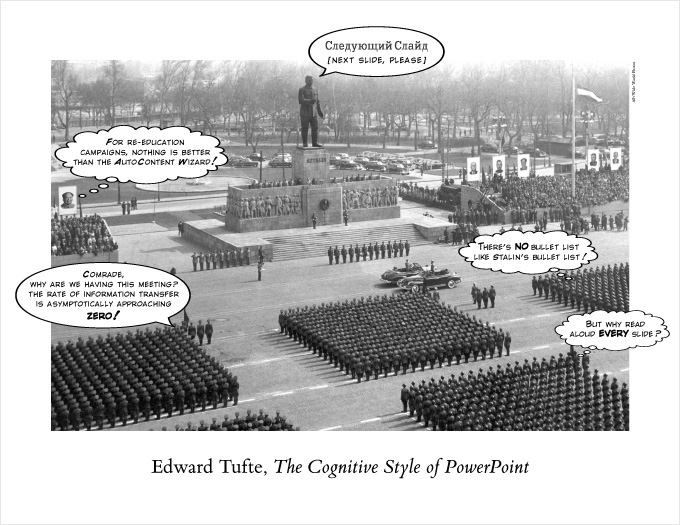
\includegraphics{../Figs/home_stalin_poster}
%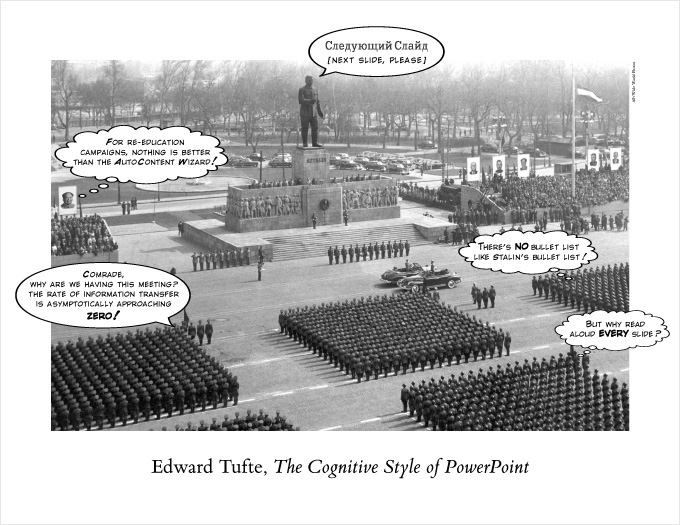
\includegraphics[width=1.0\textwidth]{../Figs/home_stalin_poster}

\begin{figure}[h!]
	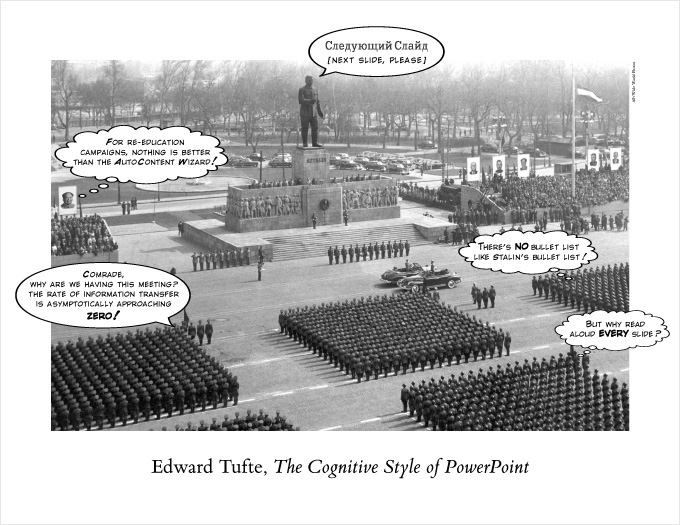
\includegraphics[width=1.0\textwidth]{../Figs/home_stalin_poster}
	\caption{No is bullet list like Stalin's bullet list}
\end{figure}

\subsection{Tables}

Do not mention the war! \citep{Cruijssen2010}
\begin{table}
	\caption{A great table}
	\label{tab: greattable}
	\centering
\begin{tabular}{ccc}
	\hline  
	1 & 2  & 3 \\ 
	\hline  
	red & yellow  & blue \\ 
	\hline 
\end{tabular} 
\end{table}

And now we refer back to our great Table \ref{tab: greattable}.


\section{Conclusion}

%\bibliographystyle{plain}
\bibliographystyle{apalike}
\bibliography{Temp}

\end{document}
